\documentclass[sigconf]{acmart}

\usepackage{booktabs} % For formal tables
\usepackage{multirow}
\usepackage[american]{babel}

% Copyright
%\setcopyright{none}
%\setcopyright{acmcopyright}
%\setcopyright{acmlicensed}
\setcopyright{rightsretained}
%\setcopyright{usgov}
%\setcopyright{usgovmixed}
%\setcopyright{cagov}
%\setcopyright{cagovmixed}


% DOI
\acmDOI{10.475/123_4}

% ISBN
\acmISBN{123-4567-24-567/08/06}

%Conference
\acmConference[WOODSTOCK'97]{ACM Woodstock conference}{July 1997}{El
  Paso, Texas USA}
\acmYear{1997}
\copyrightyear{2016}

\acmPrice{15.00}


\begin{document}
\title{Deep Transfer Bug Localization}
\titlenote{Produces the permission block, and
  copyright information}


%\author{Ben Trovato}
%\authornote{Dr.~Trovato insisted his name be first.}
%\orcid{1234-5678-9012}
%\affiliation{%
%  \institution{Institute for Clarity in Documentation}
%  \streetaddress{P.O. Box 1212}
%  \city{Dublin}
%  \state{Ohio}
%  \postcode{43017-6221}
%}
%\email{trovato@corporation.com}
%
%\author{G.K.M. Tobin}
%\authornote{The secretary disavows any knowledge of this author's actions.}
%\affiliation{%
%  \institution{Institute for Clarity in Documentation}
%  \streetaddress{P.O. Box 1212}
%  \city{Dublin}
%  \state{Ohio}
%  \postcode{43017-6221}
%}
%\email{webmaster@marysville-ohio.com}
%
%\author{Lars Th{\o}rv{\"a}ld}
%\authornote{This author is the
%  one who did all the really hard work.}
%\affiliation{%
%  \institution{The Th{\o}rv{\"a}ld Group}
%  \streetaddress{1 Th{\o}rv{\"a}ld Circle}
%  \city{Hekla}
%  \country{Iceland}}
%\email{larst@affiliation.org}
%
%\author{Valerie B\'eranger}
%\affiliation{%
%  \institution{Inria Paris-Rocquencourt}
%  \city{Rocquencourt}
%  \country{France}
%}
%\author{Aparna Patel}
%\affiliation{%
% \institution{Rajiv Gandhi University}
% \streetaddress{Rono-Hills}
% \city{Doimukh}
% \state{Arunachal Pradesh}
% \country{India}}
%\author{Huifen Chan}
%\affiliation{%
%  \institution{Tsinghua University}
%  \streetaddress{30 Shuangqing Rd}
%  \city{Haidian Qu}
%  \state{Beijing Shi}
%  \country{China}
%}
%
%\author{Charles Palmer}
%\affiliation{%
%  \institution{Palmer Research Laboratories}
%  \streetaddress{8600 Datapoint Drive}
%  \city{San Antonio}
%  \state{Texas}
%  \postcode{78229}}
%\email{cpalmer@prl.com}
%
%\author{John Smith}
%\affiliation{\institution{The Th{\o}rv{\"a}ld Group}}
%\email{jsmith@affiliation.org}
%
%\author{Julius P.~Kumquat}
%\affiliation{\institution{The Kumquat Consortium}}
%\email{jpkumquat@consortium.net}
%
%% The default list of authors is too long for headers}
%\renewcommand{\shortauthors}{B. Trovato et al.}


\begin{abstract}
This paper provides a sample of a \LaTeX\ document which conforms,
somewhat loosely, to the formatting guidelines for
ACM SIG Proceedings.\footnote{This is an abstract footnote}
\end{abstract}

%
% The code below should be generated by the tool at
% http://dl.acm.org/ccs.cfm
% Please copy and paste the code instead of the example below.
%
\begin{CCSXML}
<ccs2012>
 <concept>
  <concept_id>10010520.10010553.10010562</concept_id>
  <concept_desc>Computer systems organization~Embedded systems</concept_desc>
  <concept_significance>500</concept_significance>
 </concept>
 <concept>
  <concept_id>10010520.10010575.10010755</concept_id>
  <concept_desc>Computer systems organization~Redundancy</concept_desc>
  <concept_significance>300</concept_significance>
 </concept>
 <concept>
  <concept_id>10010520.10010553.10010554</concept_id>
  <concept_desc>Computer systems organization~Robotics</concept_desc>
  <concept_significance>100</concept_significance>
 </concept>
 <concept>
  <concept_id>10003033.10003083.10003095</concept_id>
  <concept_desc>Networks~Network reliability</concept_desc>
  <concept_significance>100</concept_significance>
 </concept>
</ccs2012>
\end{CCSXML}

\ccsdesc[500]{Computer systems organization~Embedded systems}
\ccsdesc[300]{Computer systems organization~Redundancy}
\ccsdesc{Computer systems organization~Robotics}
\ccsdesc[100]{Networks~Network reliability}


\keywords{ACM proceedings, \LaTeX, text tagging}


\maketitle

\section{Introduction}

Introduction is presented here.

\section{Background}
Background is presented here.

\section{Our Method}
The goal of cross-project bug localization is using data from source project and a few data from target project to locate the potentially buggy source code in the target project that produce the program behaviors specified in a
given bug report. Let $\mathcal{C}_s =\{ c_{s_1}, c_{s_2}, \cdots, c_{s_{nc_1}}\}$ and $\mathcal{C}_t =\{ c_{t_1}, c_{t_2}, \cdots, c_{t_{nc_2}}\}$ denote the set of source code from source project and target project respectively, $\mathcal{C}=\mathcal{C}_s \bigcup \mathcal{C}_t $. $\mathcal{R}_s =\{ r_{s_1}, r_{s_2}, \cdots, r_{s_{nr_1}}\}$ and $\mathcal{R}_t =\{ r_{t_1}, r_{t_2}, \cdots, r_{t_{nr_1}}\}$ denotes the bug reports, respectively, $\mathcal{R}=\mathcal{R}_s \bigcup \mathcal{R}_t $, where $nc_1, nc_2, nr_1, nr_2$ denote the number of source files and bug reports from source project and target project, respectively. We formulate cross-project bug localization as a learning task which aims to learn a prediction function $f: \mathcal{R} \times \mathcal{C} \mapsto \mathcal{Y}$. $y_{ij} \in \mathcal{Y} = \{+1, -1 \}$ indicates whether a source code $c_j \in \mathcal{C} $ is relevant to a bug report $r_i \in \mathcal{R}$.

In this paper, we propose a novel deep transfer neural network named TRANP-CNN (TRAnsfer Natural and Programm Language Convolutional Neural Network) to instantiate the cross-project bug localization problem, which is an extension of NP-CNN proposed by Huo et al. TRANP-CNN takes the raw data of bug reports and source code as inputs and learns a unified feature mapping $\phi(\cdot, \cdot)$ for a given $r_i$ and $c_j$, based on which the prediction can be made with a subsequent output layer. We will introduce the general framework of TRANP-CNN and explain the way to employ deep transfer technique for cross-project bug localization in the following subsections.

\subsection{General Structure}
The general framework of TRANP-CNN is shown in Figure~\ref{fig:framework}. Specifically, TRANP-CNN consists of four parts: input layer, within-project feature extraction layers, cross-project feature fusion layers and output layers. During the training process, pairs of source code and bug reports and their relevant labels from source project are fed into the deep neural network, as well as very few data from target project, and the model is trained iteratively to optimize the training loss. For testing process, a new bug report from target project containing bugs and its candidate source code are fed into the model, which outputs their relevant scores indicating which code have high relevance to the given bug report and are located as buggy.

\begin{figure*}[hbt]
\centering
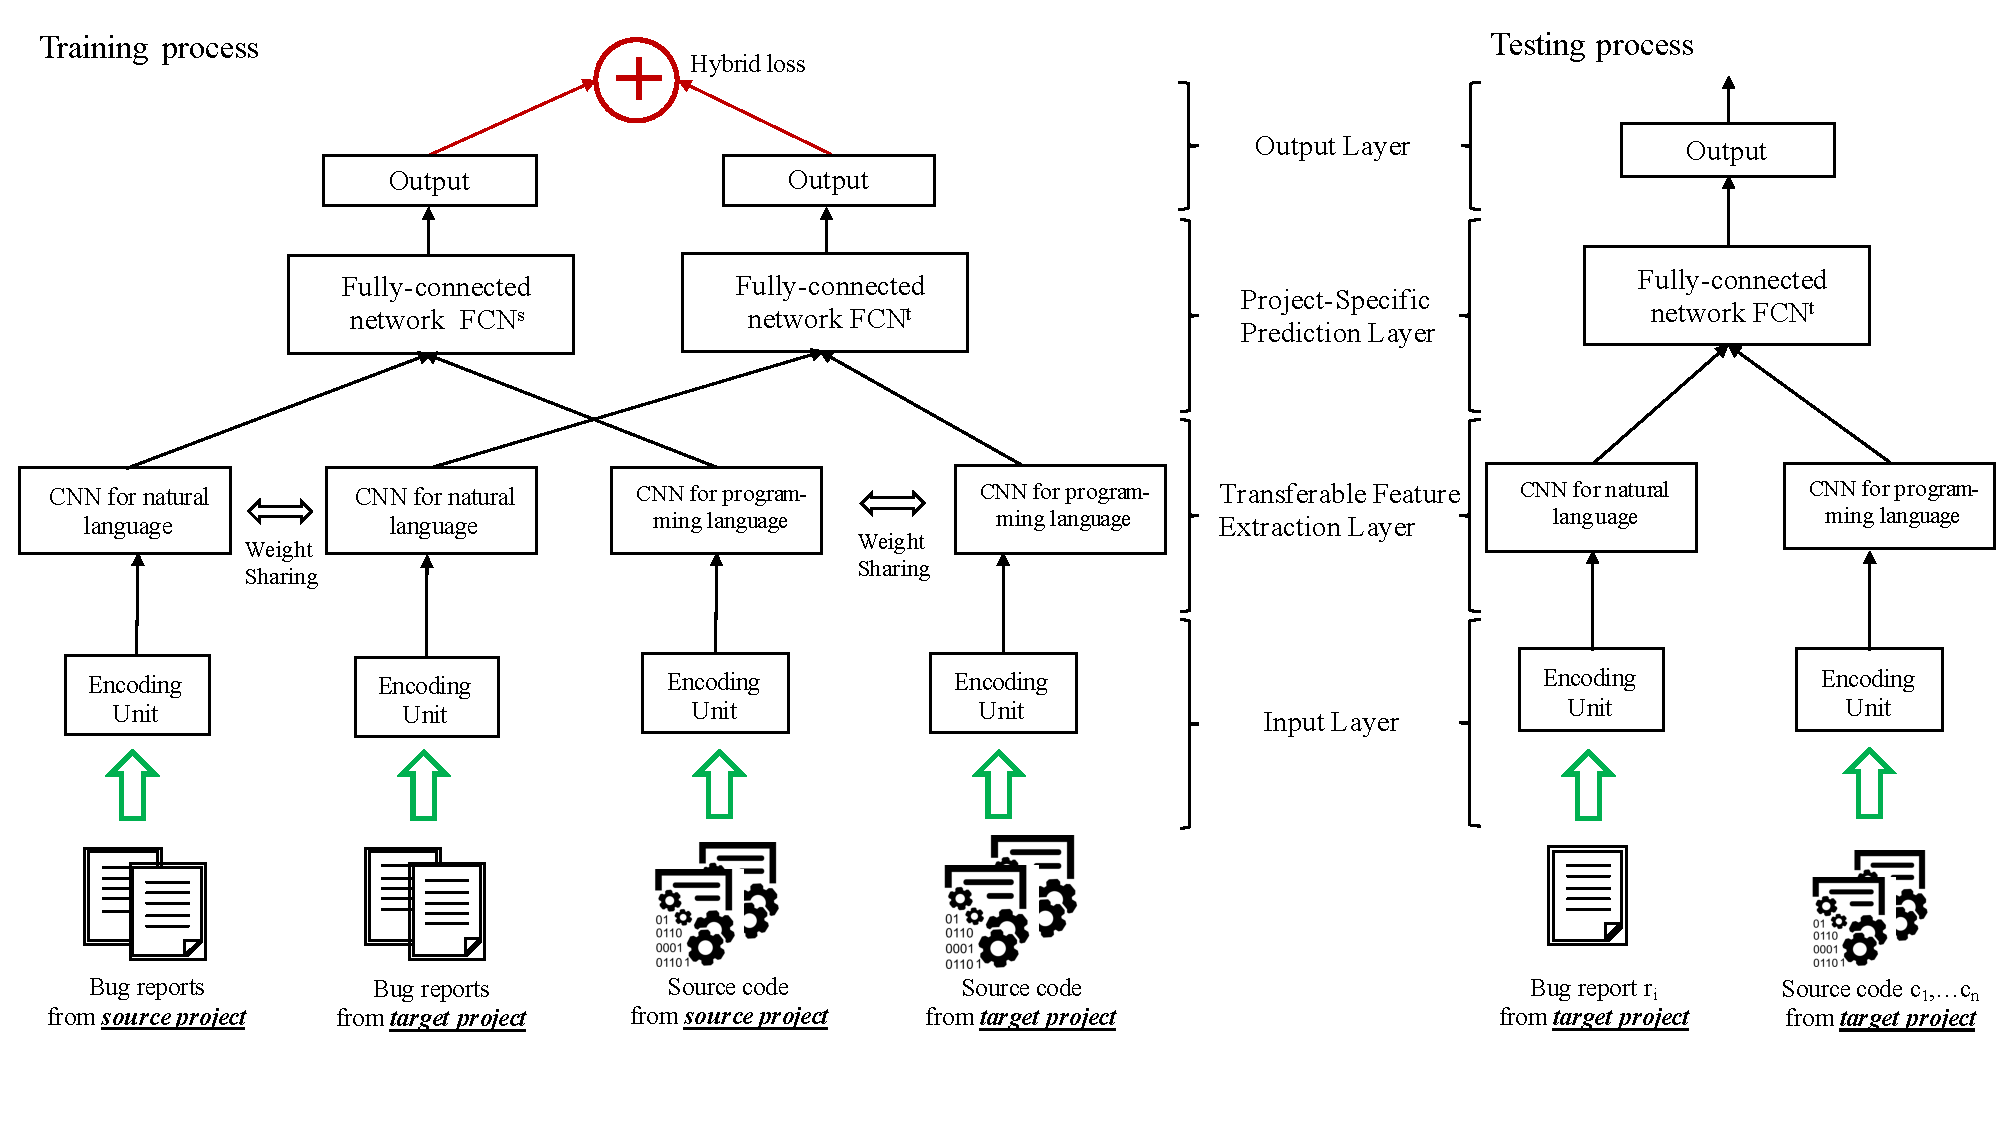
\includegraphics[width = 2\columnwidth]{pic/structure.pdf}
\caption{The overall structure of Transfer Natural and Programming language CNN. }
\label{fig:framework}
\end{figure*}

\subsection{Within-project Feature Extraction Layers}
Before processing in Within-project Feature Extraction layers, the source code and bug reports should be firstly encoded as feature vectors. Traditional techniques usually employs TFIDF to represent text content, which may lose the structural and sequential relationships between words and statements. In our model, to maintain the semantics with structural information of text, we apply word2vec technique to encode bug reports and source code.

To process the bug reports in natural language, we follow the standard approach~\cite{kim2014convolutional} to extract semantic features $\mathbf{h}^r$ from bug reports, which has been widely studied. As mentioned in Huo et al.~\cite{huo2016learning}, bug reports and source code should be processed in different ways, because two languages have different structural semantic property.

Source code in programming language, although in textural format, differs from natural language mainly in two aspects. First, the basic language component carrying meaningful semantics in natural language is word or term, and the semantics of the natural language can be inferred from a bag of words. By contrast, in programming language the basic language component carrying meaningful semantics is statement, and the semantics of the programming language can be inferred from the semantics on multiple statements plus the way how these statements interact with each other along the execution path. Thus, to extract features from programming language, the convolution operations should explicitly respect to the atomicity of statements in semantics. Second, natural language organizes words in a ``flat'' way while programming language organizes its statements in a ``structured'' way to produce richer semantics. For example, a branching structure ``if-then-else'' defines two parallel groups of statements. Each group interacts with the statements before and after the branching block while there is no interaction between the two groups. Thus, to extract features from programming language, the convolution operations should obey the program structure defined by the programming languages.

\subsection{Cross-project Feature Fusion Layers}
After processing from Within-Project Feature Extraction layers, the high-level semantic features from bug reports and source code are extracted, which would be then fed into a fully-connected neural network for feature fusion. However, in cross-project bug localization, the data distribution of source project and target project is different, which means directly employing the same fully-connected network to fuse features from both source and target projects will have bias, leading to a poor bug localization performance.

One question arises here: can we design a particular network to extract features within project, and fuse feature in separate structure? To address this problem, we design two particular fully-connected networks to combine the middle-level features in Cross-project feature fusion layers: One fully-connected network $fc_s$ is used for source project feature fusion and the other fully-connected work $fc_t$ is used to fuse features in the target project. The structure suggests that the feature extraction of different projects are similar and can be processed in the same Convolutional Neural Network, and the feature fusion and projection process is different so that two separate fully-connected neural network are designed to solve this problem. The objective function in the cross-project feature fusion layers can be rewritten in Eq.~(\ref{eq:lossfunction}):
\begin{equation}
\begin{aligned}
\label{eq:lossfunction}
\mathop{\arg\min}_{\mathbf{W}}&\sum_{s_i,s_j}\mathcal{L}(\mathbf{h}_{s_i},\mathbf{h}_{s_j}
,y_{s_{ij}}; W_{fc_s}, W_{conv} ))\\
+&\sum_{t_i,t_j}\mathcal{L}(\mathbf{h}_{t_i},\mathbf{h}_{t_j},y_{t_{ij}}; W_{fc_t}, W_{conv})+\lambda||\mathbf{W}||^2
\end{aligned}
\end{equation}
where, $\mathcal{L}$ is the square loss, $\lambda$ is the trade-off parameter and the weight vectors $W$ contains the weight vectors in convolutional neural networks $W_{conv}$, in fully-connected network of source domain $W_{fc_s}$ and in fully-connected network of target domain $W_{fc_t}$. All the weights is learned by minimizing the objective function based on SGD (stochastic gradient descent) in the same time. 


%cross-language feature fusion layers, where a fully-connected network is employed for learning a unified features and followed by an output layer mapping to the predictions $\mathcal{Y}$. However, a reported bug may only relevant to one or a few source code, while a large number of source code are irrelevant and this imbalance nature should be considered. Similar to~\cite{huo2016learning} which introduced an unequal misclassification cost to handle imbalance problem, we randomly drop some negative instances in the cross-language feature fusion layer, which can decrease the computational cost and counteract the negative influence of the imbalance nature. Let $y_{i}^{(k)}$ denote the $k$-th label of instance $\mathbf{x}_i$ and $\tilde{y}_{i}^{(k)}$ denote its prediction, similar to traditional LSTM model, we use cross entropy error function in the output layer, and the parameters are learned by minimizing the following loss function using stochastic gradient descent (SGD) method:

\section{Experiments}
To evaluate the effectiveness of TRANP-CNN, we conduct experiments on open source software projects and compare it with several state-of-the-art bug localization methods.

\subsection{Research Questions}
Our experiments are designed to address the following research questions:

\textit{\textbf{RQ1}: Is there a need for cross-project bug localization?}

\textit{\textbf{RQ2}: Does the cross-project feature fusion layer improve the bug localization performance?}

\textit{\textbf{RQ3}: Can TRANP-CNN outperform other bug localization methods?}

\subsection{Data Sets}
The data sets are presented here.

\subsection{Evaluation Metrics}
The evaluation metrics are presented here.

\subsection{Compared Methods}
We compare our proposed model TRANP-CNN with following baseline methods:
\begin{itemize}
  \item VSM (Vector Space Model)~\cite{rao2011retrieval}: a baseline method that firstly uses Vector Space Model to represent the text bug reports and source code, then employs Logistic Regression to predict the related buggy source code.
  \item Burak (Burak Filter)~\cite{peters2013better}: a state-of-the-art method for cross-project and cross-company defect prediction problem, which filters training sets using Burak filter that employs k-nearest neighbour to selects instances in the source project similar to the test project.
  \item TCA-R (Transfer Component Analysis with Logistic Regression): a state-of-the-art transfer learning method in software engineering, which firstly employ TCA to map source and target project into a same feature space and then apply Logistic Regression for bug localization (same settings suggested in their paper).
  \item TCA-P (Transfer Component Analysis with Multi-layer Perceptron): a state-of-the-art transfer learning method in software engineering, which firstly employ TCA to map source and target project into a same feature space and then apply MLPs for bug localization (same settings with fully-connected layers in TRANP-CNN).
   \item TCA-D (Transfer Component Analysis with Deep features): a state-of-the-art transfer learning method in software engineering, which firstly employ TCA to map source and target project into a same feature space and then apply Logistic Regression for bug localization (using deep features extracted from CNN instead of TFIDF features).
  \item NP-CNN (Natural and Programming language Convolutional Neural Network)~\cite{huo2016learning}: a state-of-the-art deep model for bug localization, which use source project data for training and localizing the buggy source code for target project data.
  \item SimpleTrans (Simple Transfer): a variant of the TRANP-CNN model, which trains the prediction model on the source project data, and use fine tune method for weight adjustment based on the target project.
\end{itemize}

\subsection{Experimental Settings}
For parameter settings of baseline methods, we use the same parameter settings suggested in their work~\cite{rao2011retrieval}. For the TRANP-CNN model, we employ the most commonly used ReLU $\sigma(x)=\max(0,x)$ as active function and the filter windows size $d$ is set as 3, 4, 5, with 100 feature maps each in Within-Project feature extraction layers. The number of neurons in fully-connect network in  set the same number of CNN. In addition, the drop-out method is also applied which is used to prevent co-adaption of hidden units by randomly dropping out values in fully-connected layers, and the drop-out probability $p$ is set 0.25 in our experiments.

For data partition, we use data from source projects and 20\% target projects as training sets, and locates the 80\% buggy code in target projects. This process repeats for 5 times to reduce the influence of randomness, and we report the average results in the next section.

\section{Experimental Results}

\subsection{Experimental Results for Research Questions}

\begin{table}[htbp]
  \centering
  \caption{Performance Comparisons between within-project and cross-project bug localization.}
  \resizebox{!}{0.5\columnwidth}{
    \begin{tabular}{c|l|c|c|c|c|c}
    \toprule
    Tasks & \textit{Methods} & \multicolumn{1}{l}{\textit{Top 1}} & \multicolumn{1}{l}{\textit{Top 5}} & \multicolumn{1}{l}{\textit{Top 10}} & \multicolumn{1}{l}{\textit{MAP}} & \multicolumn{1}{l}{\textit{MRR}} \\
    \midrule
    \multirow{3}[0]{*}{\textbf{J}$\rightarrow$\textbf{H}} & NPCNN & 0.317  & 0.362  & 0.508  & 0.276  & 0.352  \\
          & NPCNN$^{partial}$ & 0.204  & 0.258  & 0.313  & 0.202  & 0.292  \\
          & NPCNN$^{full}$ & 0.533  & 0.617  & 0.650  & 0.472  & 0.580  \\
          \midrule
    \multirow{3}[0]{*}{\textbf{L}$\rightarrow$\textbf{H}} & NPCNN & 0.142  & 0.192  & 0.345  & 0.161  & 0.218  \\
          & NPCNN$^{partial}$ & 0.204  & 0.258  & 0.313  & 0.202  & 0.292  \\
          & NPCNN$^{full}$ & 0.533  & 0.617  & 0.650  & 0.472  & 0.580  \\
          \midrule
    \multirow{3}[0]{*}{\textbf{H}$\rightarrow$\textbf{J}} & NPCNN & 0.167  & 0.287  & 0.349  & 0.247  & 0.277  \\
          & NPCNN$^{partial}$ & 0.035  & 0.211  & 0.302  & 0.155  & 0.189  \\
          & NPCNN$^{full}$ & 0.508  & 0.587  & 0.679  & 0.462  & 0.557  \\
          \midrule
    \multirow{3}[0]{*}{\textbf{L}$\rightarrow$\textbf{J}} & NPCNN & 0.152  & 0.182  & 0.318  & 0.176  & 0.221  \\
          & NPCNN$^{partial}$ & 0.035  & 0.211  & 0.302  & 0.155  & 0.189  \\
          & NPCNN$^{full}$ & 0.508  & 0.587  & 0.679  & 0.462  & 0.557  \\
          \midrule
    \multirow{3}[0]{*}{\textbf{H}$\rightarrow$\textbf{L}} & NPCNN & 0.173  & 0.246  & 0.390  & 0.196  & 0.329  \\
          & NPCNN$^{partial}$ & 0.097  & 0.219  & 0.335  & 0.095  & 0.109  \\
          & NPCNN$^{full}$ & 0.289  & 0.484  & 0.611  & 0.287  & 0.387  \\
          \midrule
    \multirow{3}[0]{*}{\textbf{J}$\rightarrow$\textbf{L}} & NPCNN & 0.110  & 0.255  & 0.323  & 0.141  & 0.176  \\
          & NPCNN$^{partial}$ & 0.097  & 0.219  & 0.335  & 0.095  & 0.109  \\
          & NPCNN$^{full}$ & 0.289  & 0.484  & 0.611  & 0.287  & 0.387  \\
          \midrule
    \multirow{3}[0]{*}{Avg.} & NPCNN & 0.177  & 0.254  & 0.372  & 0.200  & 0.262  \\
          & NPCNN$^{partial}$ & 0.112  & 0.229  & 0.317  & 0.151  & 0.197  \\
          & NPCNN$^{full}$ & 0.443  & 0.563  & 0.647  & 0.407  & 0.508  \\
          \bottomrule
    \end{tabular}%
    }
    
  \label{tab:within}%
\end{table}%



\textbf{RQ1}: \textit{Is there a need for cross-project bug localization?}

To answer this research question, we compare the results of using NP-CNN for bug localization in different settings.

\begin{itemize}
  \item NPCNN: Employ NPCNN directly for cross-project bug localization, which means directly training the model on the data from source projects and locating the bugs in the target project.
  \item NPCNN$^{partial}$: Employ NPCNN using partial data of target projects, which means training based on a few data (20\%) in the target projects, and localizes target buggy files without using data from source project.
  \item NPCNN$^{full}$: Employ NPCNN using full data of target projects. In this setting, we conduct 5-folds cross-validation for comparison.
\end{itemize}

The results are detailed in Tab.~\ref{tab:within}. There are six tasks in the table, in which $\textbf{H}$ represents project \textit{httpclient}, $\textbf{J}$ represents project \textit{jackrabbit} and $\textbf{L}$ represents \textit{lucene-solr}. Meanwhile, the task $\textbf{H} \rightarrow \textbf{J}$ represents using \textit{httpclient} as source project and predicts the location of buggy files in target project \textit{jackrabbit}. The results show that the performance of bug localization using full data of target projects is the best, which has a large gap against the performance using partial data. For cross-project bug localization, the performance of NPCNN that directly uses source projects is better than NPCNN$^{within}$, showing that cross-project data is beneficial to improve the bug localization performance, but directly using within-project bug localization technique will not as well as NPCNN$^{full}$. The results suggest that there is a need for cross-project bug localization, and directly using within-project bug localization method does not show good performance.

\textbf{RQ2}: \textit{Does the cross-project feature fusion layer improve the bug localization performance?}

To answer this research question, we compare the results of TRANP-CNN with NPCNN and SimpleTrans (Simple Transfer). The difference of the structure between TRANP-CNN and NPCNN is that TRANP-CNN employs two fully-connected networks to combine deep features from source projects and target projects in the cross-project feature fusion layers, respectively, which will counter the influences that cross-project data may have different distribution leading to a bias performance. The results are detailed in Tab.~\ref{tab:results2}.

According to the results, we find that SimpleTrans improves a little performance against NPCNN, showing that transfer technique is effective in improving cross-project bug localization performance. Meanwhile, it can be obviously found that TRANP-CNN performs better than NPCNN and SimpleTrans in terms of all evaluation metrics, which shows that the structure of cross-project feature fusion layer is able to improve cross-project bug localization performance.

\begin{table}[htbp]
  \centering
  \caption{Performance Comparisons with previous deep models.}
  \resizebox{!}{0.5\columnwidth}{
    \begin{tabular}{c|l|c|c|c|c|c}
    \toprule
    Tasks & \textit{Methods} & \textit{Top 1} & \textit{Top 5} & \textit{Top 10} & \textit{MAP} & \textit{MRR} \\
    \midrule
    \multirow{3}[0]{*}{\textbf{J}$\rightarrow$\textbf{H}} & NPCNN & 0.317  & 0.362  & 0.508  & 0.276  & 0.352  \\
          & SimpleTrans & 0.354 & 0.396 & 0.563 & 0.298 & 0.395 \\
          & TRANP-CNN & 0.500   & 0.583 & 0.625 & 0.376 & 0.543 \\
          \midrule
    \multirow{3}[0]{*}{\textbf{L}$\rightarrow$\textbf{H}} & NPCNN & 0.142  & 0.192  & 0.345  & 0.161  & 0.218  \\
          & SimpleTrans & 0.163 & 0.146 & 0.354 & 0.141 & 0.246 \\
          & TRANP-CNN & 0.275 & 0.35  & 0.488 & 0.242 & 0.332 \\
          \midrule
    \multirow{3}[0]{*}{\textbf{H}$\rightarrow$\textbf{J}} & NPCNN & 0.167  & 0.287  & 0.349  & 0.247  & 0.277  \\
          & SimpleTrans & 0.133 & 0.324 & 0.365 & 0.273 & 0.301 \\
          & TRANP-CNN & 0.396 & 0.443 & 0.514 & 0.371 & 0.434 \\
          \midrule
    \multirow{3}[0]{*}{\textbf{L}$\rightarrow$\textbf{J}} & NPCNN & 0.152  & 0.182  & 0.318  & 0.176  & 0.221  \\
          & SimpleTrans & 0.144 & 0.204 & 0.382 & 0.247 & 0.249 \\
          & TRANP-CNN & 0.460  & 0.462 & 0.488 & 0.404 & 0.478 \\
          \midrule
    \multirow{3}[0]{*}{\textbf{H}$\rightarrow$\textbf{L}} & NPCNN & 0.173  & 0.246  & 0.390  & 0.196  & 0.329  \\
          & SimpleTrans & 0.197 & 0.323 & 0.426 & 0.152 & 0.313 \\
          & TRANP-CNN & 0.361 & 0.445 & 0.535 & 0.279 & 0.414 \\
          \midrule
    \multirow{3}[0]{*}{\textbf{J}$\rightarrow$\textbf{L}} & NPCNN & 0.110  & 0.255  & 0.323  & 0.141  & 0.176  \\
          & SimpleTrans & 0.140  & 0.282 & 0.342 & 0.163 & 0.224 \\
          & TRANP-CNN & 0.301 & 0.410  & 0.517 & 0.247 & 0.368 \\
          \midrule
    \multirow{3}[0]{*}{Avg.} & NPCNN & 0.177  & 0.254  & 0.372  & 0.200  & 0.262  \\
          & SimpleTrans & 0.189  & 0.279  & 0.405  & 0.212  & 0.288  \\
          & TRANP-CNN & 0.382  & 0.449  & 0.528  & 0.320  & 0.428  \\
          \bottomrule
    \end{tabular}%
    }
  \label{tab:results2}%
\end{table}%

The results show that TRANP-CNN performs better than NP-CNN and SimpleTrans, which suggests that the cross-projects feature fusion layers can improve the performance of cross-projects bug localization.

\textbf{RQ3}: \textit{Can TRANP-CNN outperform other bug localization methods?}

To answer this research question, we compare the results of TRANP-CNN with state-of-the-art methods: VSM (Vector Space Model), Burak (Burak Filter), TCA-R (Transfer Component Analysis with Logistic Regression), TCA-P (Transfer Component Analysis with Multi-layer Perceptron). Vector Space Model is a baseline technique used in the within-project bug localization and we employ it on cross-project bug localization for comparison. Burak and TCA have been shown good performance on cross-project and cross-company defect prediction, and also we apply it on cross-project bug localization. The parameters are set suggested in their work, i.e., $k=2$ in Burak method, and for TCA, we implement the algorithm with TCA+. For fair comparison, the classifier in their original paper (Logistic Regression) and multi-layer perception (same as TRANP-CNN) is compared in our experiments. The results are detailed in Tab.~\ref{tab:results3}.

According to the results, we have several findings: 1. Burak and TCA techniques perform better than the baseline VSM model, indicating that using transfer algorithms is able to improve the performance in cross-project bug localization; 2. TRANP-CNN outperforms TCA-P, which shows that the high-level features extracted from CNN are more semantic and informative, leading to a better representation and bug localization performance; 3. TCA-D uses deep features extracted from CNN and the performance is not as well as TRANP-CNN, which further proves that the cross-project feature fusion layers improve bug localization performance; 4. TRANP-CNN obtains the best average values in terms of all evaluation metrics, suggesting that TRANP-CNN outperforms other traditional bug localization methods and transfer techniques on software engineering.


% Table generated by Excel2LaTeX from sheet 'Sheet3'
\begin{table}[htbp]
  \centering
  \caption{Performance comparisons with traditional bug localization performance.}
  \resizebox{!}{0.9\columnwidth}{
    \begin{tabular}{c|l|c|c|c|c|c}
    \toprule
    Tasks & \textit{Methods} & \multicolumn{1}{c|}{\textit{Top 1}} & \multicolumn{1}{c|}{\textit{Top 5}} & \multicolumn{1}{c|}{\textit{Top 10}} & \multicolumn{1}{c|}{\textit{MAP}} & \multicolumn{1}{c}{\textit{MRR}} \\
    \midrule
    \multirow{6}[0]{*}{\textbf{J}$\rightarrow$\textbf{H}} & VSM   & 0.098  & 0.157  & 0.177  & 0.087  & 0.143  \\
          & Burak & 0.110  & 0.126  & 0.138  & 0.116  & 0.121  \\
          & TCA-R & 0.120  & 0.212  & 0.144  & 0.157  & 0.162  \\
          & TCA-P & 0.114  & 0.133  & 0.154  & 0.123  & 0.176  \\
          & TCA-D & 0.122  & 0.225  & 0.271  & 0.168  & 0.248  \\
          & TRANP-CNN & 0.500  & 0.583  & 0.625  & 0.376  & 0.543  \\
          \midrule
    \multirow{6}[0]{*}{\textbf{L}$\rightarrow$\textbf{H}} & VSM   & 0.059  & 0.098  & 0.237  & 0.099  & 0.112  \\
          & Burak & 0.113  & 0.203  & 0.242  & 0.143  & 0.143  \\
          & TCA-R & 0.120  & 0.188  & 0.244  & 0.151  & 0.158  \\
          & TCA-P & 0.128  & 0.200  & 0.252  & 0.161  & 0.167  \\
          & TCA-D & 0.102  & 0.237  & 0.367  & 0.161  & 0.202  \\
          & TRANP-CNN & 0.275  & 0.350  & 0.488  & 0.242  & 0.332  \\
          \midrule
    \multirow{6}[0]{*}{\textbf{H}$\rightarrow$\textbf{J}} & VSM   & 0.035  & 0.211  & 0.232  & 0.165  & 0.129  \\
          & Burak & 0.130  & 0.150  & 0.206  & 0.225  & 0.195  \\
          & TCA-R & 0.115  & 0.162  & 0.209  & 0.239  & 0.244  \\
          & TCA-P & 0.114  & 0.154  & 0.203  & 0.237  & 0.241  \\
          & TCA-D & 0.111  & 0.135  & 0.157  & 0.168  & 0.185  \\
          & TRANP-CNN & 0.396  & 0.443  & 0.514  & 0.371  & 0.434  \\
          \midrule
    \multirow{6}[0]{*}{\textbf{L}$\rightarrow$\textbf{J}} & VSM   & 0.197  & 0.212  & 0.293  & 0.167  & 0.216  \\
          & Burak & 0.161  & 0.132  & 0.368  & 0.170  & 0.187  \\
          & TCA-R & 0.136  & 0.183  & 0.370  & 0.170  & 0.179  \\
          & TCA-P & 0.114  & 0.116  & 0.397  & 0.138  & 0.191  \\
          & TCA-D & 0.178  & 0.236  & 0.469  & 0.227  & 0.256  \\
          & TRANP-CNN & 0.460  & 0.462  & 0.488  & 0.404  & 0.478  \\
          \midrule
    \multirow{6}[0]{*}{\textbf{H}$\rightarrow$\textbf{L}} & VSM   & 0.083  & 0.278  & 0.393  & 0.154  & 0.136  \\
          & Burak & 0.105  & 0.226  & 0.272  & 0.123  & 0.222  \\
          & TCA-R & 0.136  & 0.208  & 0.383  & 0.170  & 0.279  \\
          & TCA-P & 0.143  & 0.226  & 0.394  & 0.171  & 0.288  \\
          & TCA-D & 0.162  & 0.207  & 0.345  & 0.229  & 0.292  \\
          & TRANP-CNN & 0.361  & 0.445  & 0.535  & 0.279  & 0.414  \\
          \midrule
    \multirow{6}[0]{*}{\textbf{J}$\rightarrow$\textbf{L}} & VSM   & 0.038  & 0.077  & 0.154  & 0.124  & 0.204  \\
          & Burak & 0.138  & 0.161  & 0.176  & 0.168  & 0.226  \\
          & TCA-R & 0.135  & 0.111  & 0.172  & 0.169  & 0.222  \\
          & TCA-P & 0.136  & 0.132  & 0.192  & 0.173  & 0.237  \\
          & TCA-D & 0.142  & 0.297  & 0.308  & 0.238  & 0.293  \\
          & TRANP-CNN & 0.301  & 0.410  & 0.517  & 0.247  & 0.368  \\
          \midrule
    \multirow{6}[0]{*}{Avg.} & VSM   & 0.085  & 0.172  & 0.248  & 0.133  & 0.157  \\
          & Burak & 0.126  & 0.166  & 0.234  & 0.157  & 0.182  \\
          & TCA-R & 0.127  & 0.178  & 0.254  & 0.176  & 0.207  \\
          & TCA-P & 0.125  & 0.160  & 0.265  & 0.167  & 0.217  \\
          & TCA-D & 0.136  & 0.223  & 0.319  & 0.199  & 0.246  \\
          & TRANP-CNN & 0.382  & 0.449  & 0.528  & 0.320  & 0.428  \\
          \bottomrule
    \end{tabular}%
    }
  \label{tab:results3}%
\end{table}%




\subsection{Discussions of the Results}

\subsubsection{Why do the cross-project feature fusion layers work? }

\subsubsection{Why does TRANP-CNN improve the bug localization performance?}

\section{Threats to Validity}
Threats to Validity.

\section{Relate Work}
Relate work.

\section{Conclusions}
This paragraph will end the body of this sample document.


\bibliographystyle{ACM-Reference-Format}
\bibliography{ICSE18}

\end{document}
